\begin{enunciado}{\ejercicio}
  \begin{enumerate}[label=\alph*)]
    \item Calcular $w + \conj w + (w + w^2)^2 - w^{38}(1 - w^2)$ para cada $w \en G_7$.
    \item Calcular $w^{73} + \conj w \cdot w^9 + 8$ para cada $w\en G_3$.
    \item Calcular $1 + w^2 + w^{-2} + w^4 + w^{-4}$ para cada $w\en G_{10}$.
    \item Calcular $w^{14} + w^{-8} + \conj w^4 + \conj{w^{-3}}$ para cada $w \en G_5$
  \end{enumerate}
\end{enunciado}

\textit{Voy a estar usando las siguientes propiedades en $G_n$: }\\
Si $w \en G_n \entonces
  \llave{l}{
    w^n = 1 \entonces w^k = w^{r_n(k)}                                                                         \\
    \conj w^k = w^{r_n(-k)}                                                                                    \\
    \sumatoria{k=0}{n-1}w^k = 0                                                                                \\
    m \divideA n \entonces G_m \subseteq G_n,\text{ lo uso para saber con cuales raíces hay que tener cuidado} \\
    \text{Si } w \en G_p \text{ con $p$ primo }}$\par

\begin{enumerate}[label=\alph*)]
  \item Calcular $w + \conj w + (w + w^2)^2 - w^{38}(1 - w^2)$ para cada $w \en G_7$.

        \separadorCorto
        Raíces de $G_7$ de interés: 7 es primo e impar $\entonces w = 1$ se hace a parte.\par
        \textit{Si} $w = 1$: \par
        $w + \conj w + (w + w^2)^2 - w^{38}(1 - w^2) = 6$\par

        \textit{Si} $w \distinto 1$: \\
        $w + \ub{\conj w}{w^6} + (w + w^2)^2 - w^{38}(1 - w^2) =
          w + w^6 + w^2 + 2w^3 + w^4 - \ub{(w^7)^5}{=1} w^3(1 - w^2) =\\
          =  \magenta{-1} + \ub{\magenta{1} + w + w^2 + w^3 + w^4 + w^5 + w^6}{=0} = -1 \Tilde$

  \item Calcular $w^{73} + \conj w \cdot w^9 + 8$ para cada $w\en G_3$.

        \separadorCorto
        Raíces de $G_3$ de interés: 3 es primo e impar $\entonces w = 1$ se hace a parte.\par
        \textit{Si} $w = 1$: \par
        $w^{73} + \conj w \cdot w^9 + 8 = 10 $\par

        \textit{Si} $w \distinto 1$: \\
        $\ub{w^{73}}{w} + \ub{\conj w \cdot w^9 }{w^2 \cdot 1}+ 8 =
          \magenta{-1} + \ub{\magenta{1} + w + w^2}{= 0} + 8 = 7 $

  \item Calcular $1 + w^2 + w^{-2} + w^4 + w^{-4}$ para cada $w\en G_{10}$.

        $$
          \begin{minipage}{0.55\textwidth}
            Tuneo un poco el enunciado usando que:
            $$
              w \en G_{10}
              \entonces
              w^m = w^{\magenta{r_{10}(m)}},
            $$
            por lo tanto:
            $$
              1 + w^2 + w^{-2} + w^4 + w^{-4}
              \igual{\red{!}}
              1 + w^2 + w^{\magenta{8}} + w^4 + w^{\magenta{6}}
            $$
            Todas potencias pares escribo como:
            $$
              1 + w^2 + w^{\magenta{8}} + w^4 + w^{\magenta{6}}
              \igual{\red{!}}
              \sumatoria{i = 0}{4} (w^2)^i \quad \llamada1
            $$
            Si $w = \blue{\pm 1}$, dado que $\blue{\pm 1} \en G_{10}$, $\llamada1$ queda:
            $$
              \sumatoria{i = 0}{4} (\blue{(\pm 1)}^2)^i = 5,
            $$
          \end{minipage}
          \begin{minipage}{0.3\textwidth}
            \centering
            $G_5 \subseteq G_{10}$\par
            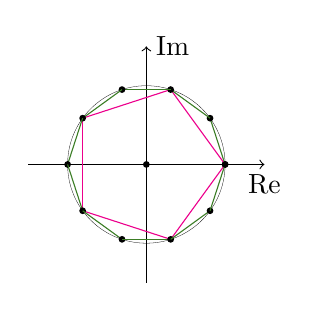
\begin{tikzpicture}[baseline=0]
              \draw[->] (-1.5,0) -- (1.5,0) node[below] {Re};
              \draw[->] (0,-1.5) -- (0,1.5) node[right] {Im};
              \draw[ultra thin] (0,0) circle (1);
              \filldraw[thin] (0,0) circle (1pt); % Added the origin
              \foreach \x in {0,...,10} {
                  \filldraw (\x*360/10:1) circle (1pt);
                  \ifnum\x<10
                    \draw[OliveGreen] (\x*360/10:1) -- ({(\x+1)*360/10}:1);
                  \fi
                  \ifnum\x<5
                    \draw[magenta] (\x*360/5:1) -- ({(\x+1)*360/5}:1);
                  \fi
                }
            \end{tikzpicture}

            $G_{10} - G_5 = "G_5" \subseteq G_{10}$

            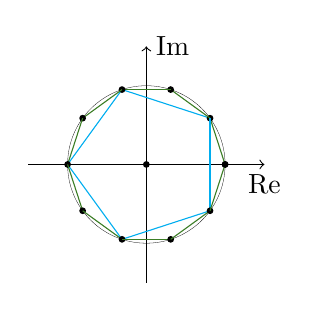
\begin{tikzpicture}[baseline=0]
              \draw[->] (-1.5,0) -- (1.5,0) node[below] {Re};
              \draw[->] (0,-1.5) -- (0,1.5) node[right] {Im};
              \draw[ultra thin] (0,0) circle (1);
              \filldraw[thin] (0,0) circle (1pt); % Added the origin

              \foreach \x in {0,...,10} {
                  \filldraw (\x*360/10:1) circle (1pt);
                  \ifnum\x<10
                    \draw[OliveGreen] (\x*360/10:1) -- ({(\x+1)*360/10}:1);
                  \fi
                  \ifnum\x<5
                    \draw[cyan] ({\x*360/5+360/10}:1) -- ({(\x+1)*360/5+360/10}:1);
                  \fi
                }
            \end{tikzpicture}
          \end{minipage}

          pero si no uso fórmula geométrica:
        $$
        \sumatoria{i = 0}{4} (w^2)^i  =
        \frac{(w^2)^{4 + 1} - 1}{w^2 - 1} =
        \frac{w^{10} - 1}{w^2 - 1} =
        \frac{\magenta{1} - 1}{w^2 - 1} = 0
        $$

  \item Calcular $w^{14} + w^{-8} + \conj w^4 + \conj{w^{-3}}$
        para cada $w \en G_5$

        \separadorCorto

        \textit{Si} $w = 1$:
        $$
          w^{14} + w^{-8} + \conj w^4 + \conj{w^{-3}} = 4
        $$
        \textit{Si} $w \distinto 1$:
        $$
          w^{14} + w^{-8} + \conj w^4 + \conj{w^{-3}} =
          w^4 + w^2 + w + w^3 =
          \magenta{-1} + \ub{\magenta{1} + w + w^2 + w^3 + w^4}{= 0} = -1
        $$
\end{enumerate}

\begin{aportes}
  \item \aporte{\dirRepo}{naD GarRaz \github}
\end{aportes}
